\hypertarget{ia-e-analuxedtica-industrial}{%
\chapter{IA e Analítica Industrial}\label{ia-e-analuxedtica-industrial}}

\section*{Objetivos de Aprendizagem}

Ao final deste capítulo, o leitor será capaz de:

\begin{itemize}
\tightlist
\item
  Distinguir as quatro famílias de problema que a analítica industrial resolve.
\item
  Verificar se os dados de uma planta estão prontos para um modelo --- antes de contratá-lo.
\item
  Estruturar um projeto de manutenção preditiva e de detecção de anomalia.
\item
  Descrever o ciclo de vida de um modelo industrial, do treino ao retreino.
\item
  Reconhecer os modos de falha de um modelo em operação e os limites do seu uso.
\end{itemize}

\begin{center}\rule{0.5\linewidth}{0.5pt}\end{center}

\hypertarget{o-que-a-induxfastria-realmente-pede-uxe0-ia}{%
\section{O que a indústria realmente pede à IA}\label{o-que-a-induxfastria-realmente-pede-uxe0-ia}}

``Aplicar inteligência artificial'' não é um problema de engenharia --- é um guarda-chuva. Na prática, os
pedidos se organizam em quatro famílias, e cada uma tem pré-requisito diferente:

\textbf{Tabela 20.1 -- As quatro famílias de problema}

\begin{longtable}[]{@{}
  >{\raggedright\arraybackslash}p{(\columnwidth - 6\tabcolsep) * \real{0.2500}}
  >{\raggedright\arraybackslash}p{(\columnwidth - 6\tabcolsep) * \real{0.2500}}
  >{\raggedright\arraybackslash}p{(\columnwidth - 6\tabcolsep) * \real{0.2500}}
  >{\raggedright\arraybackslash}p{(\columnwidth - 6\tabcolsep) * \real{0.2500}}@{}}
\toprule\noalign{}
\begin{minipage}[b]{\linewidth}\raggedright
Família
\end{minipage} & \begin{minipage}[b]{\linewidth}\raggedright
Pergunta que responde
\end{minipage} & \begin{minipage}[b]{\linewidth}\raggedright
Exemplo industrial
\end{minipage} & \begin{minipage}[b]{\linewidth}\raggedright
Pré-requisito principal
\end{minipage} \\
\midrule\noalign{}
\endhead
\bottomrule\noalign{}
\endlastfoot
Classificação & ``Isto é A ou B?'' & Peça conforme ou não conforme; motor em falha ou normal & Exemplos \textbf{rotulados} de cada classe \\
Regressão (sensor virtual) & ``Quanto vale o que eu não meço?'' & Estimar qualidade em linha a partir de variáveis medidas & Relação estável entre entrada e saída \\
Detecção de anomalia & ``Isto está diferente do normal?'' & Comportamento atípico de conjunto motobomba & \emph{Baseline} de operação normal, bem definido \\
Otimização & ``Qual o melhor ajuste agora?'' & Reduzir consumo de energia mantendo a produção & Modelo do processo e função objetivo acordada \\
\end{longtable}

O erro mais comum de projeto é começar pela técnica. A ordem correta é: \textbf{definir a decisão} que será
tomada com o resultado, o \textbf{tempo disponível} para tomá-la e o \textbf{custo} de errar. Só então se escolhe
o método --- que, em boa parte dos casos industriais reais, é uma regra simples com limite bem ajustado.

\begin{center}
\IfFileExists{../figuras/capitulo-20-m1.pdf}{%
  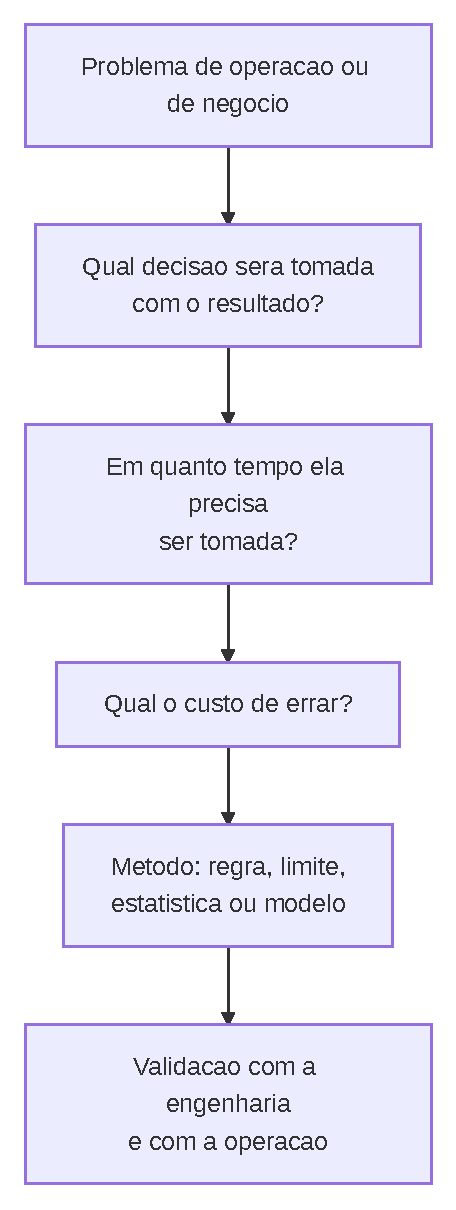
\includegraphics[width=\linewidth,height=0.8\textheight,keepaspectratio]{../figuras/capitulo-20-m1.pdf}%
}{\fbox{\parbox{0.9\linewidth}{\small Diagrama Mermaid ainda não renderizado: capitulo-20-m1. Rode scripts/render-mermaid.sh.}}}
\end{center}

\begin{center}\rule{0.5\linewidth}{0.5pt}\end{center}

\hypertarget{o-pruxe9-requisito-dado-com-contexto}{%
\section{O pré-requisito: dado com contexto}\label{o-pruxe9-requisito-dado-com-contexto}}

Nenhuma técnica compensa dado mal formado. Antes de qualquer modelo, quatro verificações:

\begin{enumerate}
\def\labelenumi{\arabic{enumi}.}
\tightlist
\item
  \textbf{Tag com significado completo} --- nome estável, unidade, faixa, contexto e qualidade
  (Capítulos 14 e 15).
\item
  \textbf{Histórico com resolução adequada ao fenômeno} --- um modelo de vibração treinado com amostra de
  30 s não enxerga nada (Capítulo 16).
\item
  \textbf{Eventos de falha registrados} --- com data, hora, equipamento e \textbf{causa}. Sem causa registrada,
  não existe rótulo, e sem rótulo não existe classificação.
\item
  \textbf{Contexto operacional} --- regime de carga, produto sendo fabricado, turno, temperatura ambiente.
  Um modelo treinado em um regime e aplicado em outro aprendeu a reconhecer o regime, não a falha.
\end{enumerate}

\begin{caixaatencao}

\textbf{Atenção:} o gargalo mais frequente não é o algoritmo, é a \textbf{ordem de serviço}. Em muitas
plantas, o registro de manutenção diz ``bomba 2 --- defeito'' sem informar qual componente falhou.
Sem essa informação, o histórico técnico mais rico da empresa é inútil para aprendizado
supervisionado. Corrigir o formulário de manutenção é, literalmente, o primeiro passo do projeto de
IA --- e o mais barato.

\end{caixaatencao}

\begin{caixafigura}

\textbf{{[}Figura 20.1 -- Diagnóstico de prontidão dos dados para analítica{]}}
\emph{Painel de verificação com quatro blocos de semáforo: cobertura de tags (percentual de variáveis com unidade, faixa e qualidade definidas), resolução do histórico (variáveis com taxa de amostragem compatível com o fenômeno), registro de eventos (número de paradas com causa documentada no último ano) e rotulagem (proporção de ocorrências de manutenção com componente identificado). Abaixo, uma lista dos dez ativos prioritários com o bloco que falta em cada um.}

\end{caixafigura}

\begin{center}\rule{0.5\linewidth}{0.5pt}\end{center}

\hypertarget{manutenuxe7uxe3o-preditiva}{%
\section{Manutenção preditiva}\label{manutenuxe7uxe3o-preditiva}}

A manutenção evolui em níveis, e cada nível exige mais dado que o anterior:

\textbf{Tabela 20.2 -- Níveis de manutenção}

\begin{longtable}[]{@{}
  >{\raggedright\arraybackslash}p{(\columnwidth - 6\tabcolsep) * \real{0.2500}}
  >{\raggedright\arraybackslash}p{(\columnwidth - 6\tabcolsep) * \real{0.2500}}
  >{\raggedright\arraybackslash}p{(\columnwidth - 6\tabcolsep) * \real{0.2500}}
  >{\raggedright\arraybackslash}p{(\columnwidth - 6\tabcolsep) * \real{0.2500}}@{}}
\toprule\noalign{}
\begin{minipage}[b]{\linewidth}\raggedright
Nível
\end{minipage} & \begin{minipage}[b]{\linewidth}\raggedright
Quando se intervém
\end{minipage} & \begin{minipage}[b]{\linewidth}\raggedright
Dado necessário
\end{minipage} & \begin{minipage}[b]{\linewidth}\raggedright
Limitação
\end{minipage} \\
\midrule\noalign{}
\endhead
\bottomrule\noalign{}
\endlastfoot
Corretiva & Depois da falha & Nenhum & Parada não planejada e dano secundário \\
Preventiva & Por calendário ou horas de operação & Contador de horas & Troca de componente bom e falha entre intervalos \\
Baseada em condição & Quando um indicador cruza um limite & Vibração, corrente, temperatura, análise de óleo & Depende de limite bem escolhido e de tendência confiável \\
Preditiva & Quando a projeção indica falha em janela útil & Série histórica com eventos rotulados & Exige histórico longo e disciplina de registro \\
Prescritiva & Antes, com recomendação de ação & Modelo de degradação e de custo & Depende de confiabilidade do modelo e de confiança da operação \\
\end{longtable}

Os sinais de campo que alimentam a análise são conhecidos e não exigem instrumentação exótica: valor
eficaz de vibração e sua decomposição em faixas, temperatura de mancal, corrente do motor e seu
desvio do padrão, pressão diferencial, análise periódica de óleo. O que faz diferença não é o sensor,
é a \textbf{tendência com baseline}: a mesma leitura de vibração significa coisas diferentes em máquinas
diferentes e em regimes diferentes.

\begin{caixadica}

\textbf{Dica:} comece pela manutenção \textbf{baseada em condição} com limites extraídos do próprio
histórico, antes de partir para modelos preditivos. Ela entrega resultado em semanas, exige só o que
já existe e --- o mais importante --- estabelece a disciplina de registro que o modelo preditivo vai
precisar depois.

\end{caixadica}

\begin{caixafigura}

\textbf{{[}Figura 20.2 -- Tendência de indicador de condição com desvio progressivo{]}}
\emph{Gráfico de linha com a evolução de um indicador de vibração ao longo de seis meses, com faixa de referência sombreada (baseline com dispersão) e uma linha de limite de atenção. No início do período a curva oscila dentro da faixa; a partir de determinado ponto inicia subida gradual, cruza o limite de atenção e continua. Anotar na figura o início da subida, o cruzamento do limite e o instante da intervenção, mostrando a janela de antecedência obtida.}

\end{caixafigura}

\begin{center}\rule{0.5\linewidth}{0.5pt}\end{center}

\hypertarget{detecuxe7uxe3o-de-anomalia}{%
\section{Detecção de anomalia}\label{detecuxe7uxe3o-de-anomalia}}

Detecção de anomalia é a técnica mais promissora para a indústria, e a mais fácil de arruinar. Três
distinções precisam estar claras:

\begin{itemize}
\tightlist
\item
  \textbf{Anomalia não é falha.} Um comportamento diferente pode ser um regime novo, um produto diferente
  ou uma condição de clima. Anomalia é convite à investigação, não alarme.
\item
  \textbf{Limite estático \ensuremath{\times} dinâmico.} Um limite fixo é simples, previsível, auditável e frequentemente
  suficiente. Um modelo multivariável captura interações que o limite fixo não vê --- e cobra o preço em
  explicabilidade.
\item
  \textbf{O inimigo é o falso positivo.} Um detector que avisa dez vezes por dia é desligado na segunda
  semana. O mesmo raciocínio de racionalização de alarmes do Capítulo 10 se aplica: se ninguém age, o
  aviso não deveria existir.
\end{itemize}

\begin{center}
\IfFileExists{../figuras/capitulo-20-m2.pdf}{%
  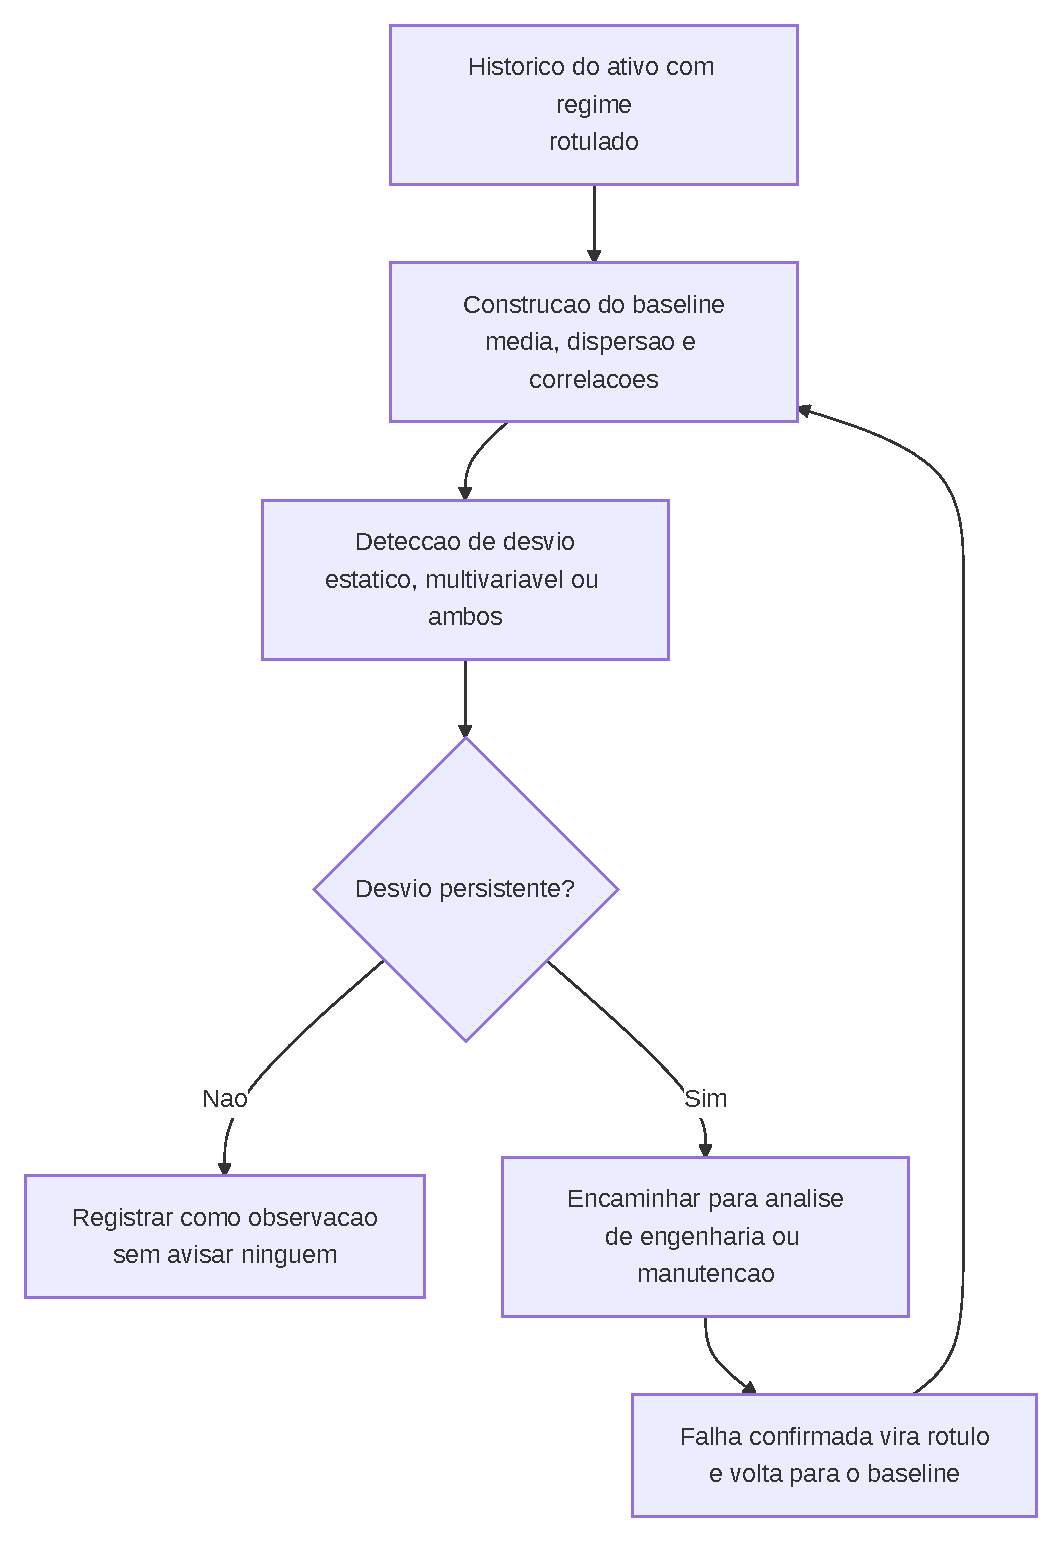
\includegraphics[width=\linewidth,height=0.8\textheight,keepaspectratio]{../figuras/capitulo-20-m2.pdf}%
}{\fbox{\parbox{0.9\linewidth}{\small Diagrama Mermaid ainda não renderizado: capitulo-20-m2. Rode scripts/render-mermaid.sh.}}}
\end{center}

O último passo do diagrama é o que separa um projeto vivo de um projeto abandonado: \textbf{a falha
confirmada volta como rótulo}. Sem esse retorno, o sistema não aprende e o detector continua com o
mesmo desempenho do primeiro dia --- ou pior, porque o processo mudou.

\begin{center}\rule{0.5\linewidth}{0.5pt}\end{center}

\hypertarget{sensor-virtual-e-controle-avanuxe7ado}{%
\section{Sensor virtual e controle avançado}\label{sensor-virtual-e-controle-avanuxe7ado}}

Duas aplicações de regressão que pagam bem o investimento:

\begin{itemize}
\tightlist
\item
  \textbf{Sensor virtual} (\emph{soft sensor}): estimar em tempo real uma variável que só é medida em
  laboratório ou por analisador de alto custo, a partir de variáveis medidas continuamente. Aplicação
  típica em qualidade de produto. Requisito: a relação entre entrada e saída precisa ser estável o
  suficiente, e o modelo precisa saber dizer quando está fora da sua região de validade.
\item
  \textbf{Controle avançado}: usar um modelo do processo para calcular a ação considerando restrições e
  horizonte futuro --- o que já era feito, sem aprendizado de máquina, pelo controle preditivo baseado
  em modelo (MPC). Aqui, a contribuição da analítica está em manter o modelo atualizado e em detectar
  quando ele deixa de representar o processo.
\end{itemize}

Em ambos os casos, a saída do modelo \textbf{orienta} a decisão; ela não escreve diretamente no atuador sem
malha de segurança. Usar uma predição como \emph{setpoint} de proteção é confundir previsão com garantia.

\begin{center}\rule{0.5\linewidth}{0.5pt}\end{center}

\hypertarget{o-ciclo-de-vida-do-modelo-em-operauxe7uxe3o}{%
\section{O ciclo de vida do modelo em operação}\label{o-ciclo-de-vida-do-modelo-em-operauxe7uxe3o}}

Um modelo industrial não termina no treino. Ele tem ciclo de vida, e o ciclo tem modos de falha
próprios.

\textbf{Tabela 20.3 -- Etapas do ciclo e os modos de falha}

\begin{longtable}[]{@{}
  >{\raggedright\arraybackslash}p{(\columnwidth - 4\tabcolsep) * \real{0.3333}}
  >{\raggedright\arraybackslash}p{(\columnwidth - 4\tabcolsep) * \real{0.3333}}
  >{\raggedright\arraybackslash}p{(\columnwidth - 4\tabcolsep) * \real{0.3333}}@{}}
\toprule\noalign{}
\begin{minipage}[b]{\linewidth}\raggedright
Etapa
\end{minipage} & \begin{minipage}[b]{\linewidth}\raggedright
O que se faz
\end{minipage} & \begin{minipage}[b]{\linewidth}\raggedright
Como falha
\end{minipage} \\
\midrule\noalign{}
\endhead
\bottomrule\noalign{}
\endlastfoot
Preparação & Seleção de variáveis, tratamento de lacunas e de valores ruins & Misturar períodos com configuração diferente sem marcá-los \\
Treino e validação & Ajuste do modelo e verificação em dados não usados no treino & Vazamento de dados: treinar e validar no mesmo período \\
Implantação & Publicação do resultado onde a decisão acontece & Modelo certo no lugar errado --- resultado em painel que ninguém abre \\
Monitoramento & Vigilância do erro e das entradas & Ninguém percebe que a variável de entrada mudou de comportamento \\
Deriva e retreino & Atualização com dado novo & Retreinar sem revisar: o modelo aprende a nova condição anormal como normal \\
\end{longtable}

A \textbf{deriva} (\emph{drift}) é o modo de falha mais silencioso. Ela acontece por três caminhos: o processo
muda (equipamento reformado, produto novo), o sensor muda (descalibração, substituição por outro
modelo) ou a relação muda (a causa deixou de ser a mesma). Nas três, o sintoma na tela é o mesmo:
o modelo continua respondendo, com confiança, errado.

\begin{caixanota}

\textbf{Nota:} um modelo em produção é um \textbf{ativo com prazo de validade}, e precisa de dono, de
indicador de desempenho e de rotina de revisão. Modelo sem dono é passivo técnico: fica na planta
até alguém descobrir, em uma investigação de acidente, que a recomendação vinha de um sistema
treinado com dados de quatro anos antes.

\end{caixanota}

\begin{caixafigura}

\textbf{{[}Figura 20.3 -- Painel de acompanhamento de um modelo em operação{]}}
\emph{Captura de painel com quatro blocos: desempenho do modelo ao longo do tempo (acerto e falsos positivos por mês), distribuição das variáveis de entrada comparada com a do treino, número de recomendações emitidas e quantas geraram intervenção, e lista das últimas recomendações com o desfecho registrado. Destacar o bloco de desvio de entrada, que é o alerta antecipado de deriva.}

\end{caixafigura}

\begin{center}\rule{0.5\linewidth}{0.5pt}\end{center}

\hypertarget{limites-e-riscos}{%
\section{Limites e riscos}\label{limites-e-riscos}}

\textbf{Tabela 20.4 -- Riscos e a resposta de engenharia}

\begin{longtable}[]{@{}
  >{\raggedright\arraybackslash}p{(\columnwidth - 4\tabcolsep) * \real{0.3333}}
  >{\raggedright\arraybackslash}p{(\columnwidth - 4\tabcolsep) * \real{0.3333}}
  >{\raggedright\arraybackslash}p{(\columnwidth - 4\tabcolsep) * \real{0.3333}}@{}}
\toprule\noalign{}
\begin{minipage}[b]{\linewidth}\raggedright
Risco
\end{minipage} & \begin{minipage}[b]{\linewidth}\raggedright
Descrição
\end{minipage} & \begin{minipage}[b]{\linewidth}\raggedright
Resposta
\end{minipage} \\
\midrule\noalign{}
\endhead
\bottomrule\noalign{}
\endlastfoot
Correlação tratada como causa & O modelo aprende que a parada vem junto com um evento que é consequência dela & Validar com engenharia de processo; nunca concluir causa a partir do modelo \\
Opacidade & Ninguém sabe explicar a recomendação & Preferir modelos interpretáveis quando a decisão for crítica \\
Viés de registro & Só falhas que já eram observadas estão rotuladas & Reconhecer o limite; não usar o modelo como detector do desconhecido \\
Uso fora do domínio & Aplicar em equipamento ou regime não representado no treino & Declarar a região de validade e recusar a resposta fora dela \\
Uso para segurança & Colocar predição no caminho de proteção & Proibido: proteção é do SIS e do intertravamento (Capítulos 8 e 15) \\
Custo invisível & O modelo melhora o indicador e piora a operação & Medir o efeito na planta, não só a métrica do modelo \\
\end{longtable}

\begin{caixaatencao}

\textbf{Atenção:} IA e analítica não substituem proteção, intertravamento nem sistema de segurança
instrumentado. Um modelo estatístico não tem nível de integridade de segurança, não é certificado
para função de proteção e não responde em tempo determinístico. Ele ajuda a decidir; não protege
pessoas nem ativos.

\end{caixaatencao}

\begin{center}\rule{0.5\linewidth}{0.5pt}\end{center}

\hypertarget{estudo-de-caso-o-modelo-que-acertava-e-ninguuxe9m-usava}{%
\section{\texorpdfstring{Estudo de Caso --- O modelo que acertava e ninguém usava}{Estudo de Caso  O modelo que acertava e ninguém usava}}\label{estudo-de-caso-o-modelo-que-acertava-e-ninguuxe9m-usava}}

\textbf{Cenário.} Uma planta de celulose contratou o desenvolvimento de um modelo preditivo de falha para
os motores do setor de bombas. O modelo foi entregue com 91 \% de acerto na validação, sobre um
histórico de três anos de vibração e corrente. A recomendação chegava por painel em nuvem.

\textbf{Diagnóstico.} Seis meses depois, a manutenção não havia mudado uma única intervenção por causa do
modelo. Três motivos:

\begin{enumerate}
\def\labelenumi{\arabic{enumi}.}
\tightlist
\item
  \textbf{A decisão não passou pelo modelo.} O planejamento da manutenção é semanal; a recomendação
  chegava por painel, sem entrar na rotina do planejador.
\item
  \textbf{A região de validade não era dita.} Metade dos avisos vinha de dois motores que operavam em
  regime intermitente, ausente do histórico de treino.
\item
  \textbf{O retorno de rótulo não existia.} As falhas confirmadas nunca voltaram para o modelo, e as
  substituições preventivas --- que evitam a falha --- não foram registradas como tal, o que fazia o
  modelo parecer pior do que era.
\end{enumerate}

\textbf{Decisão de engenharia.}

\begin{longtable}[]{@{}
  >{\raggedright\arraybackslash}p{(\columnwidth - 2\tabcolsep) * \real{0.5000}}
  >{\raggedright\arraybackslash}p{(\columnwidth - 2\tabcolsep) * \real{0.5000}}@{}}
\toprule\noalign{}
\begin{minipage}[b]{\linewidth}\raggedright
Problema
\end{minipage} & \begin{minipage}[b]{\linewidth}\raggedright
Medida
\end{minipage} \\
\midrule\noalign{}
\endhead
\bottomrule\noalign{}
\endlastfoot
Modelo fora da rotina & Recomendação injetada como item no plano semanal de manutenção, com justificativa e prioridade \\
Região de validade ignorada & Motores em regime intermitente separados em outro grupo, com baseline próprio \\
Sem retorno de rótulo & O registro de manutenção passou a exigir causa e componente; o resultado alimenta o retreino \\
Sem medição de resultado & Indicador de falsos positivos por mês e de acertos que geraram intervenção \\
\end{longtable}

\textbf{Resultado.} No semestre seguinte, 11 intervenções foram antecipadas por recomendação do modelo, com
redução de paradas não planejadas. O acerto do modelo não mudou --- o que mudou foi o sistema em torno
dele: a recomendação entrou na rotina, a região de validade foi respeitada e o resultado passou a ser
medido.

\textbf{Limitações do arranjo.} O modelo continua dependendo de um baseline revisado a cada mudança de
configuração de processo. E os motores em regime intermitente seguem com desempenho inferior, porque
o histórico disponível para eles é curto --- limitação de dado, não de método.

\begin{center}\rule{0.5\linewidth}{0.5pt}\end{center}

\hypertarget{resumo}{%
\section{Resumo}\label{resumo}}

\begin{itemize}
\tightlist
\item
  A indústria pede quatro coisas distintas: \textbf{classificação, regressão, detecção de anomalia e otimização} --- cada uma com pré-requisito próprio.
\item
  O projeto começa pela \textbf{decisão} a ser tomada e pelo custo de errar, não pela técnica.
\item
  Dado com \textbf{contexto} (unidade, faixa, qualidade, regime, causa registrada) é pré-requisito; corrigir o formulário de manutenção costuma ser o primeiro passo.
\item
  A manutenção evolui de corretiva a prescritiva; a \textbf{baseada em condição} já entrega resultado e prepara o terreno.
\item
  \textbf{Anomalia não é falha}; o inimigo do detector é o falso positivo, e o mesmo raciocínio de racionalização de alarmes se aplica.
\item
  A \textbf{falha confirmada precisa voltar como rótulo}, ou o sistema não aprende.
\item
  Sensor virtual e controle avançado orientam a decisão; não escrevem no atuador sem malha de segurança.
\item
  Modelo em produção \textbf{tem prazo de validade}, dono, indicador e rotina de revisão --- a deriva é o modo de falha mais silencioso.
\item
  \textbf{IA não substitui proteção, intertravamento nem SIS}; não tem nível de integridade de segurança.
\end{itemize}

\hypertarget{questuxf5es-de-revisuxe3o}{%
\section{Questões de Revisão}\label{questuxf5es-de-revisuxe3o}}

\begin{enumerate}
\def\labelenumi{\arabic{enumi}.}
\tightlist
\item
  Descreva as quatro famílias de problema da analítica industrial e dê um exemplo de cada em uma planta de sua escolha.
\item
  Por que a definição da decisão deve preceder a escolha do método? Ilustre com um caso em que uma regra simples resolve o problema.
\item
  Liste quatro verificações de prontidão dos dados e explique o que cada uma impede.
\item
  Por que a ausência de causa no registro de manutenção inviabiliza aprendizado supervisionado? Como corrigir isso na prática?
\item
  Compare manutenção baseada em condição e manutenção preditiva quanto a dado necessário e limitação.
\item
  Explique a diferença entre anomalia e falha, e por que o excesso de avisos leva ao abandono do sistema.
\item
  Descreva o ciclo de vida de um modelo industrial e um modo de falha de cada etapa.
\item
  O que é deriva de modelo, quais os três caminhos que a produzem e como detectá-la?
\item
  Explique por que um modelo com 91 \% de acerto pode não gerar nenhum benefício. Cite três causas organizacionais.
\item
  Justifique tecnicamente por que um modelo de aprendizado de máquina não pode substituir o sistema de segurança instrumentado de uma planta.
\end{enumerate}

\hypertarget{referuxeancias}{%
\section{Referências}\label{referuxeancias}}

\begin{itemize}
\tightlist
\item
  VIANNA, W. S. \textbf{IIoT e suas Tecnologias Aderentes: Teoria e exemplos práticos}. Material didático do curso (Indústria 4.0, inteligência artificial, aprendizado de máquina e tecnologias aderentes).
\item
  VIANNA, W. S. \textbf{Introdução a IoT}. Material didático do curso (aprendizado de máquina e análise avançada sobre dados de dispositivos; plataformas de nuvem).
\item
  ORACLE. \textbf{O que é IoT} --- conceitos de Internet das Coisas, conectividade e análise. Disponível em: \url{oracle.com/br/internet-of-things}. Consulta: 2026 (referência citada pelo material de origem do curso).
\item
  CISCO. \textbf{An Introduction to IoT} (documento de pesquisa traduzido) --- fundamentos de IoT e conectividade. Referência citada pelo material de origem do curso.
\item
  INFLUXDATA. \textbf{InfluxDB Documentation} --- consulta e agregação para análise de séries temporais. Disponível em: docs.influxdata.com. Consulta: 2026.
\item
  GRAFANA LABS. \textbf{Grafana Documentation} --- painéis de acompanhamento de indicadores e de desempenho de modelos. Disponível em: \url{grafana.com/docs}. Consulta: 2026.
\item
  THINGSBOARD. \textbf{Documentação oficial} --- telemetria, atributos e alarmes como fonte de dado para análise. Disponível em: \url{thingsboard.io/docs}. Consulta: 2026.
\end{itemize}
